\section{Training HighRes--net}
As stated in the experiment layout, the final step consists in training HighRes--net super--resolution model with different data.
One final step before conducting the training is to examine visually the results of augmentation on the Sentinel--2 image.
These are presented for the simple convolutional augmentation network architecture in the figure \ref{fig:export-example} and \ref{fig:export-example-zoomed}.
\begin{figure}
    \begin{subfigure}[t]{0.3\textwidth}
        \centering
        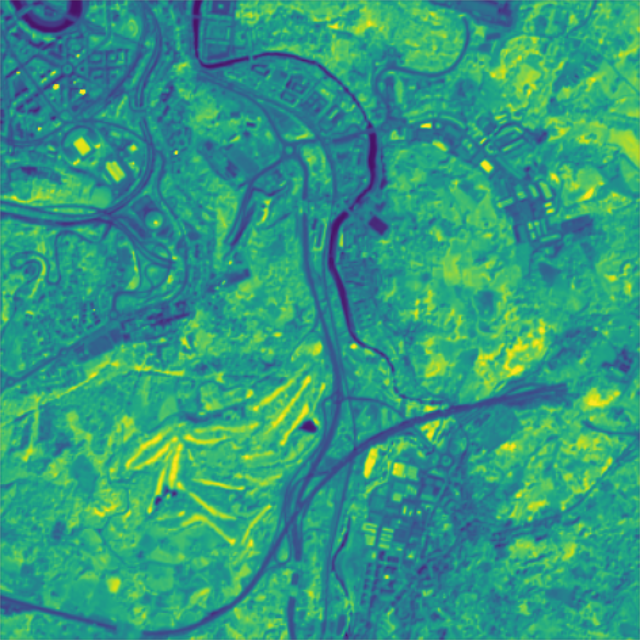
\includegraphics[width=\textwidth]{sentinel_export_hr}
        \caption{High--resolution}
    \end{subfigure}
    \hfill
    \begin{subfigure}[t]{0.3\textwidth}
        \centering
        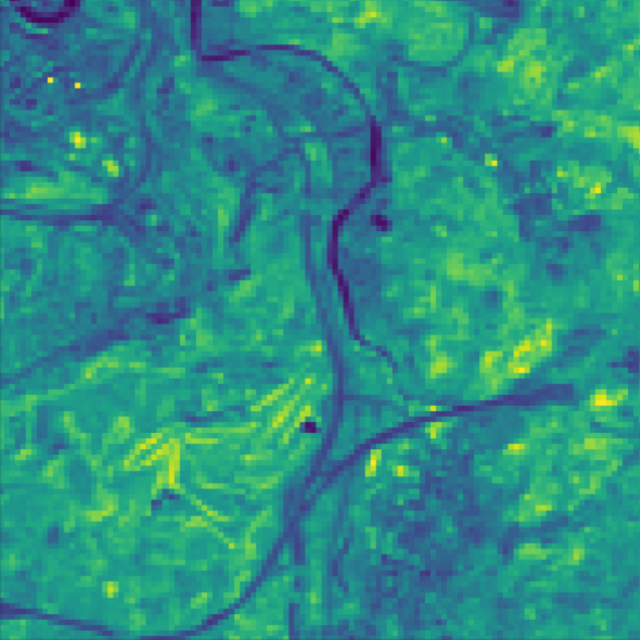
\includegraphics[width=\textwidth]{sentinel_export_pred}
        \caption{Low--resolution augmented}
    \end{subfigure}
    \hfill
    \begin{subfigure}[t]{0.3\textwidth}
        \centering
        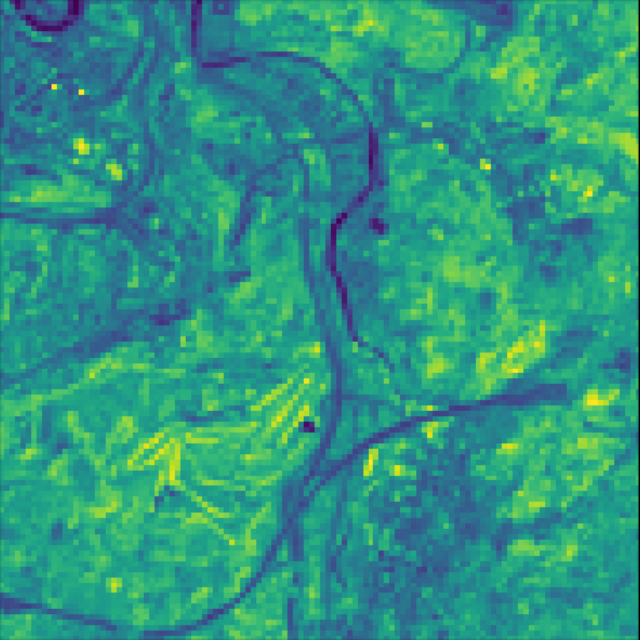
\includegraphics[width=\textwidth]{sentinel_export_bicubic}
        \caption{Low resolution resized with bicubic}
    \end{subfigure}
    \caption{Example of Sentinel--2 training data export with simple convolutional augmentation network}
    \label{fig:export-example}
\end{figure}
\begin{figure}
    \begin{subfigure}[t]{0.3\textwidth}
        \centering
        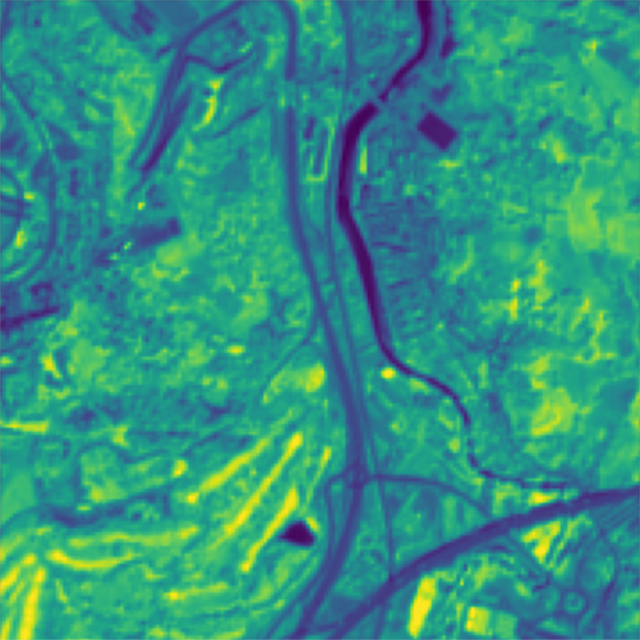
\includegraphics[width=\textwidth]{sentinel_export_zoomed_hr}
        \caption{High--resolution}
    \end{subfigure}
    \hfill
    \begin{subfigure}[t]{0.3\textwidth}
        \centering
        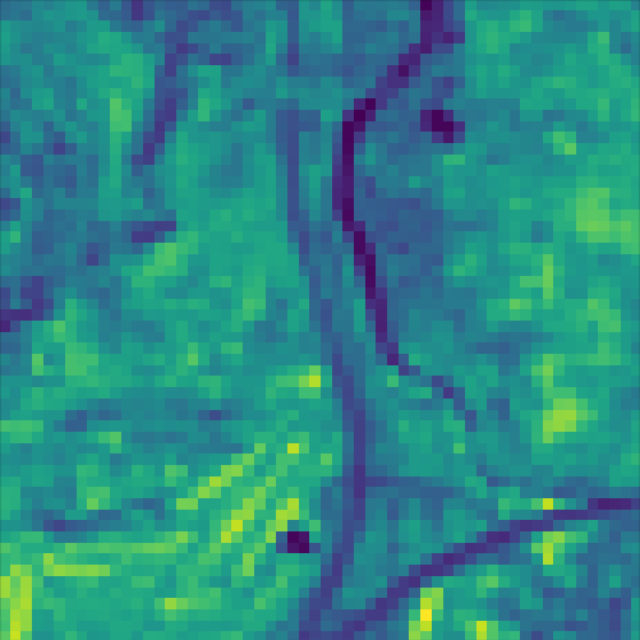
\includegraphics[width=\textwidth]{sentinel_export_zoomed_pred}
        \caption{Low--resolution augmented}
    \end{subfigure}
    \hfill
    \begin{subfigure}[t]{0.3\textwidth}
        \centering
        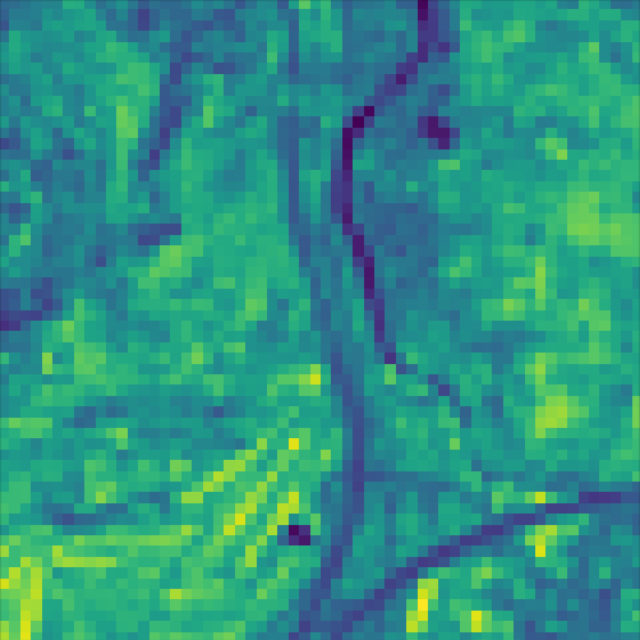
\includegraphics[width=\textwidth]{sentinel_export_zoomed_bicubic}
        \caption{Low resolution resized with bicubic}
    \end{subfigure}
    \caption{Zoomed example of Sentinel--2 training data export with simple convolutional augmentation network}
    \label{fig:export-example-zoomed}
\end{figure}

As planned, the super--resolution is to be trained with multi--image data in a single--band (eight band) mode.
Training is configured in such a way that only weights for the best validation score are saved.
However, automatic stopping is not enabled, for this reason fitting was interrupted manually around epoch one hundred when all training curves plateaued.
Training history has been plotted to visualize the loss fitting progress.

\subsection{Cross validation as stop condition}
Having multiple datasets generated in different ways enables an alternative way of validating the training process.
Instead of taking a subpart of the training set as validation data, one may use images generated in a different way.
Such a technique may help to investigate the generalization capabilities of the super--resolution network.
The dataset created using the simple convolutional network and resizing algorithm were used for the cross validation.
In each of them, one set was used for fitting and the other was used for validation.
This time the increasing validation loss indicates overfitting in early epochs, compared to previous trainings.
A small raise in validation loss is visible for over ten epochs before the training was stopped.
In this case, best weights were saved nearly three times earlier than during the non--cross--validated training. 
This may indicate that the vast part of the fitting process does not contribute to overall generalization capability of the super--resolution network.
The cross--validated training is stopped earlier; since only weights for the epoch with the best validation score are saved, it is pointless to run longer fittings.
Figure \ref{fig:highres-net-training-loss} shows the loss history for all discussed HighRes--net trainings, figure \ref{fig:highres-net-training-validation} presents validation loss improvement.
\begin{figure}
    \centering
    \begin{tikzpicture}
			\begin{axis}[width=\linewidth, height=12cm, grid=major, grid style={dashed}, xlabel=Epoch, ylabel=Loss]
			\addlegendentry{Bicubic}
			\addplot+[mark=none] table [x=step, y=value, col sep=comma] {data/highresnet_s2ab_ab5_bb8_20210608-114450-training_loss.csv};
			\addlegendentry{Simple convolutional}
						\addplot+[mark=none] table [x=step, y=value, col sep=comma] {data/highresnet_s2_degraded_simple_conv-dvc-21-07-04_044726_e34_bb8_20210706-183639-training_loss.csv};
			\addlegendentry{Encoder--decoder}
						\addplot+[mark=none] table [x=step, y=value, col sep=comma] {data/highresnet_s2_degraded_autoencoder-dvc-21-07-04-052647_e23_bb8_20210707-100146-training_loss.csv};
			\addlegendentry{GAN}
						\addplot+[mark=none] table [x=step, y=value, col sep=comma] {data/highresnet_s2_degraded-gan-dvc-21-07-04-055506_e94_bb8_20210707-152641-training_loss.csv};
			\addlegendentry{t: Bicubic, v: Simple convolutional}
						\addplot+[mark=none, color=green] table [x=step, y=value, col sep=comma] {data/highresnet_s2ab_ab5_bb8_20210726-160215-training_loss.csv};

			\end{axis}		\end{tikzpicture}
    \caption{HighRes--net training loss history}
    \label{fig:highres-net-training-loss}
\end{figure}
\begin{figure}
    \centering
    \begin{tikzpicture}
			\begin{axis}[width=\linewidth, height=12cm, grid=major, grid style={dashed}, xlabel=Epoch, ylabel=Loss]
			\addlegendentry{Bicubic}
			\addplot+[mark=none] table [x=step, y=value, col sep=comma] {data/highresnet_s2ab_ab5_bb8_20210608-114450-validation_loss.csv};
			\addlegendentry{Simple convolutional}
						\addplot+[mark=none] table [x=step, y=value, col sep=comma] {data/highresnet_s2_degraded_simple_conv-dvc-21-07-04_044726_e34_bb8_20210706-183639-validation_loss.csv};
			\addlegendentry{Encoder--decoder}
						\addplot+[mark=none] table [x=step, y=value, col sep=comma] {data/highresnet_s2_degraded_autoencoder-dvc-21-07-04-052647_e23_bb8_20210707-100146-validation_loss.csv};
			\addlegendentry{GAN}
						\addplot+[mark=none] table [x=step, y=value, col sep=comma] {data/highresnet_s2_degraded-gan-dvc-21-07-04-055506_e94_bb8_20210707-152641-validation_loss.csv};
			\addlegendentry{t: Bicubic, v: Simple convolutional}
						\addplot+[mark=none, color=green] table [x=step, y=value, col sep=comma] {data/highresnet_s2ab_ab5_bb8_20210726-160215-validation_loss.csv};

			\end{axis}		\end{tikzpicture}
    \caption{HighRes--net validation loss history}
    \label{fig:highres-net-training-validation}
\end{figure}

\section{Evaluation and results}
According to the experiment layout, the trained super--resolution models are to be evaluated on a variety of test datasets to examine generalization capabilities and robustness.
As stated before, the evaluation datasets include:
\begin{itemize}
	\item Test subsets from all augmented Sentinel--2 datasets that can be used for calculating numerical metrics.
	\item Real--life Sentinel--2 images that were not used in the training process. These do not include high and low--resolution pairs, so only visual examination can be performed.
	\item Proba--V test dataset that can be used for calculating numerical metrics.
\end{itemize}
It should be noticed that the later two test sets differ in the GSD parameter from the synthetic low--resolution images in the Sentinel--2 training datasets.
This data is still valid for evaluation and investigation because it is desirable that super--resolution, and machine learning algorithms in general, work on objects of any scale and size.
Limiting tests to single GSD would draw an incomplete picture of the results.
The results of evaluation are presented in the table \ref{tab:super-res-results}, where rows designate test datasets and columns indicate models trained on data created in different ways.
For the cross--validation training scenarios, letters \textit{t} and \textit{v} indicate training and validation datasets respectively.
The \textit{cPSNR} score was used as the super--resolution evaluation metric.

The best results are observed on the diagonal of the table, which means that the algorithm works best on test data created in the same way as training data for a given model.
This result is expected and indicates that no gross mistakes were made in the course of the work.
A visual demonstration of such an evaluation can be seen in the figure \ref{fig:highresnet-test-visual}.
An example of image upscaling with bicubic interpolation was included in the figure as a reference point.
In this case HighRes--net was trained on the dataset created by simple convolutional network and evaluated on the test subpart of the same dataset.
\begin{figure}[p]
    \centering
    \begin{subfigure}[t]{0.45\textwidth}
        \centering
        
\includegraphics[width=\textwidth]{highresnet_test_lr}
        \caption{One of nine low--resolution images}
    \end{subfigure}
    \hfill
    \begin{subfigure}[t]{0.45\textwidth}
        \centering
        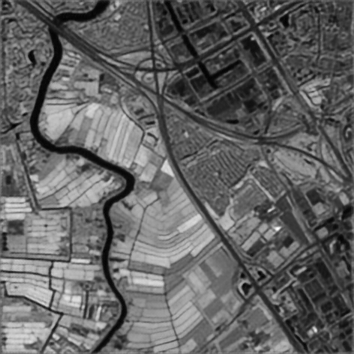
\includegraphics[width=\textwidth]{highresnet_test_sr}
        \caption{Super--resolution reconstruction of the scene}
    \end{subfigure}
    \begin{subfigure}[t]{0.45\textwidth}
        \centering
        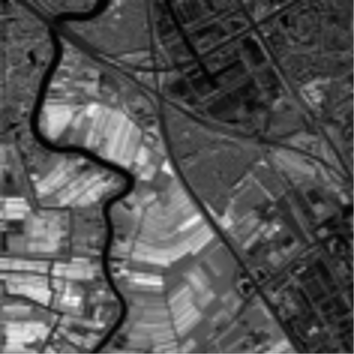
\includegraphics[width=\textwidth]{highresnet_test_bicubic}
        \caption{Upscaling to high--resolution with bicubic interpolation}
    \end{subfigure}
    \hfill
    \begin{subfigure}[t]{0.45\textwidth}
        \centering
        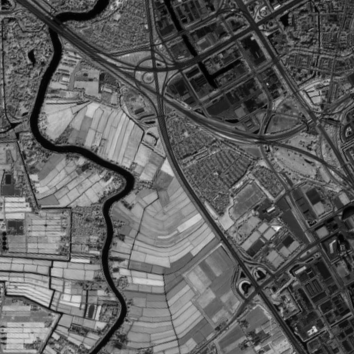
\includegraphics[width=\textwidth]{highresnet_test_hr}
        \caption{Real--life high--resolution picture of the scene}
    \end{subfigure}
    \caption{An example on evaluation of augmented dataset; both the training and test data were generated using simple convolutional network}
    \label{fig:highresnet-test-visual}
\end{figure}
\begin{table}
\caption{Evaluation of super--resolution training on different test sets}
\label{tab:super-res-results}
\begin{adjustbox}{center}
\small
\begin{tabular}{lccccc}
\toprule
cPSNR &
  Bicubic &
  Simple conv &
  Encoder--decoder &
  GAN &
  \begin{tabular}[c]{@{}c@{}}t: Bicubic\\ v: Simple convolutional\end{tabular} \\
\midrule
Bicubic                      &  35.78 & 28.96 & 24.55 & 25.80 &  35.26 \\
Simple convolutional                  & 33.69 & 36.15 & 27.16 & 29.83 & 33.67  \\
Encoder--decoder             & 31.72 & 31.78 & 34.43 & 30.22 & 31.76 \\
GAN                          & 28.63 & 28.63 & 27.27 & 35.72 &  30.28 \\
Proba--V                      & 43.36 & 42.02 & 40.43 & 40.91 & 43.51  \\
\bottomrule
\end{tabular}
\end{adjustbox}
\end{table}

As stated before, the results on the Sentinel--2 real--life image were evaluated visually by observing artifacts in the images.
This test on data with different GSD proves some issues with data generalization.
Some mosaic or checkerboard--like artifacts can be observed on the super--resolved images.
An example of such a phenomenon (generated by the best performing network trained on bicubic data with cross--validation) can be observed in the figure \ref{fig:sentinel-real-artifacts}.
\begin{figure}
	\centering
    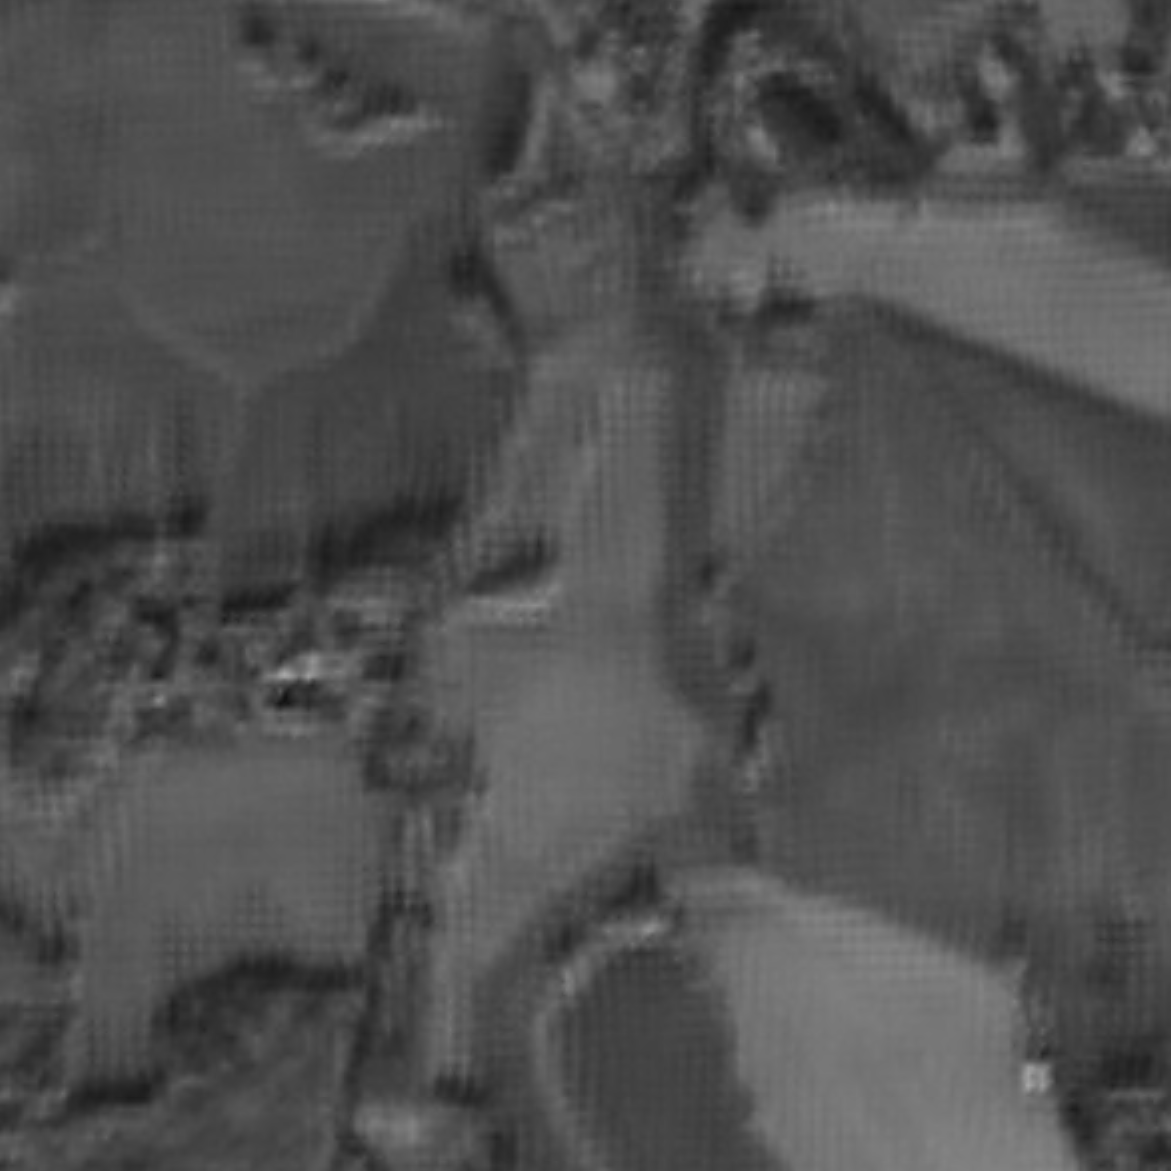
\includegraphics[width=0.7\textwidth]{sentinel_real_artifacts}
    \caption{An example of artifacts phenomenon on the Sentinel--2 real data}
    \label{fig:sentinel-real-artifacts}
\end{figure}

The results in the table \ref{tab:super-res-results} can be summarized in the following statements:
\begin{itemize}
	\item Data created with augmentation techniques, both traditional and deep learning--based is suitable for training super--resolution networks.
	\item The different deep learning architectures give fairly similar results, although the simplest one works best.
	\item At the moment, the bicubic interpolation gives slightly better results, possible reasons for that and suggestions of improvement are included in the summary.
	\item The cross--validation proves that all training are prone to overfitting to the data generation techniques. Early stopping based on different datasets can leads to this conclusion.
	\item Generalization capabilities of the networks--trained on synthetic data poses a problem. Artifacts on real data can be observed.
\end{itemize}